% \important{Analytically look into energy. Three sections -> Importance to this paper}

% There are many metrics to evaluate the environmental impact of blindly deploying embedded AI. We choose here to look at the energetic demand that the implementation of embodied AI in smart factories will bring about. To understand where this demand will come from we have isolated what we believe are three crucial challenges. In the following we discuss them individually highlighting what is the impact that they will have in future energy consumption.

% \begin{figure}[!ht]
% 	\centering
% 	\includegraphics[width=0.45\textwidth]{fig/data_centers_energy_germany.png}
% 	\caption{Germany's data centers energy demand (from \cite{hintemann2020efficiency})\TODO}
% 	\label{fig:dataCenterEnergyDE}
% \end{figure}
%%---
%IBM's Summit super computer \textcolor{red}{Summit divides work among 4,608 interconnected computer nodes housed in refrigerator-sized cabinets and liquid-cooled by pumping 4,000 gallons of water per minute through the system. It takes up an eighth of an acre -- the size of two tennis courts. Its peak energy consumption is about 15 megawatts, enough to power more than 7,000 homes. See \url{https://www.cnet.com/news/ibms-world-class-summit-supercomputer-gooses-speed-with-ai-abilities/}}
% \begin{figure*}[!t]
% 	\centering
% 	\hspace*{\fill}
% 	\subfloat[]{\includegraphics[width= 0.30\textwidth]{fig/robot_stock} \label{fig:ir_stock}}
% 	\hfill
% 	\subfloat[]{\includegraphics[width= 0.30\textwidth]{fig/robot_energy} \label{fig:ir_energy}}
% 	\hfill
% 	\subfloat[]{\includegraphics[width= 0.30\textwidth]{fig/share_industrial_and_cobots} \label{fig:industrial_cobot_share}}	
% 	\hspace*{\fill}
% 	\\[-2ex]
% 	\hspace*{\fill}
% 	\subfloat[]{\includegraphics[width= 0.3\textwidth]{fig/col_bot_stock}\label{fig:cobot_stock}}
% 	\hfill    
% 	\subfloat[]{\includegraphics[width= 0.3\textwidth]{fig/col_bot_energy}\label{fig:cobot_energy}}
% 	\hfill    
% 	\subfloat[]{\includegraphics[width= 0.3\textwidth]{fig/advanced_robots_in_manufacturing_projected_global_demand}\label{fig:advanced_robots_in_manufacturing_projected_global_demand}}
% 	\hspace*{\fill}    
% 	\caption[] {\label{fig:robot_forecasts} Forecasts for robot operational stock and energy consumption: \subref{fig:ir_stock} industrial robots install base forecast and \subref{fig:ir_energy} estimated worldwide energy consumption, \subref{fig:industrial_cobot_share} ratio of industrial to cobots,  \subref{fig:cobot_stock} cobots sales forecast and their \subref{fig:cobot_energy} estimated worldwide energy consumption, \subref{fig:advanced_robots_in_manufacturing_projected_global_demand} projected demand for advanced robotics in manufacturing worldwide between 2018 and 2021 (in billion USD).}
% \end{figure*}
% As stated before, Industry 4.0 and the smart factory will be the main contributors to the rise in robots (see Fig.~\ref{fig:advanced_robots_in_manufacturing_projected_global_demand}). However, modern technologies and lifestyle and societal needs will make robots ubiquitous permeating many aspects of human life. As a consequence the current and future additions to the population of robots will cause a, currently disregarded, increment in the demand of electric energy. By obtaining an average power consumption per robot application category, based on the information from leading robot manufacturers, estimates for the yearly \textit{World Robot Energy Consumption} were calculated. The magnitudes of these estimates rise a concern when compared to values for electricity consumption and installed generation capacity. By presenting these numbers it is intended to raise awareness on this incoming problem in order to devise strategies to tackle it.

%To our knowledge there is no research that determines the amount of energy needed to manufacture a robot. Therefore, a model is developed that transfers the numbers from the car industry (see Apex B). These estimations result in a large energy ($\unit[45]{MJ}$) and material demand ($\unit[90]{t}$) for one average robot (KUKA 240).
%In 2019 roughly $2,700,000$ robots were manufactured\footnote{See \url{https://de.statista.com/statistik/daten/studie/250212/umfrage/geschaetzter-bestand-von-industrierobotern-weltweit/}}. This corresponds to a demand of $\unit[91.8\cdot10^9]{GJ}$ which is only a small fraction to the German energy consumption ($\unit[1.8\cdot10^{18}]{J}$) and thus not yet very relevant to the overall energy consumption. Nevertheless, it can be expected that the number of robots will explode exponentially and, thus, letting the energy demand explode as well.

%\subsubsection{Apex B} %TODO push to appendix!
%As far as we know, there are no reliable numbers for the amount of energy and materials needed to manufacture a robot. Nevertheless, these numbers can be estimated by transferring them from the auto mobile manufacturing. Detailed studies report up to 34 MJ of energy for a 1.5 t car \cite{sullivan2010energy}. Other sources\footnote{See \url{https://www.vcoe.at/service/fragen-und-antworten/wie-viele-ressourcen-werden-bei-der-pkw-produktion-verbraucht}}, (\textcolor{red}{\textbf{better citation needed}}) speak of 70t of needed resources for an average car (1.5 t). It can be assumed that a car and an industry robot have the same ``complexity'' that is the ratio of materials and the same energy consumption per kg for manufacturing.
%For example considering a $\unit[2000]{kg}$ robot would result in an energy consumption of $\unit[2]{t} \cdot \frac{\unit[34]{MJ}}{\unit[1.5]{t}} =\unit[45]{MJ}$ and a material consumption of $\unit[2]{t} \cdot \frac{\unit[70]{t}}{\unit[1.5]{t}}=\unit[90]{t}$.


%\subsubsection{Methods to encounter this challenge}
%
%To overcome this challenge we propose different methods.
%
%\paragraph{Reducing the number of manufactured robots}
%The most obvious way to encounter this challenge is reducing the number of manufactered robots. This can be done in quite a few ways. The life-time cycles of the robots can be encreased, the modularity of the robots increased and more flexible robots could be developed.
%
%\paragraph{More efficient manufacturing}
%The manufacturing of the robots could be done more efficient if it is done by more efficient robots itself. Here, all of the already named methods of the 2nd challenge to reduce the energy demand for driving a robot take place as well.
%
%\paragraph{Recycling}
%The best way to save energy and materials is recycling.
%For example only 95\% of the energy is needed for recycling aluminum than processing the raw materials \cite{}. %TODO: \url{https://www.eia.gov/energyexplained/energy-and-the-environment/recycling-and-energy.php}
%Furthermore, mining often devastates the environment and has led to large environmental disasters while on the other hand, non-recycled waste needs much place in landfills and often contaminates the environment. While some materials are recycled quite completely, unfortunately until now it is especially difficult to recycle electronic waste.
%Often, this has to be done with toxic chemicals manually.\cite{}
%Automatisating this process therefore is a urgently needed step.
%
%Detailed considerations including proposing a metric, mathematical framing and detailed determining of solutions would exceed the format of this paper and will therefore be done individually in a following research project.

% Metals and minerals, for instance, are one of the most demanded materials for the manufacturing of robots for both their mechanical and electronic components. Their mining often devastates the environment and has led to large environmental disasters. Furthermore, non-recycled waste needs many places in landfills and often contaminates the environment. If, for instance, recycling is fostered, relevant energy savings can be achieved (e.g. the recycling process of aluminum only needs 95\% of the energy used to process the raw materials). On the other hand, while some materials are recycled almost completely, unfortunately until now it is especially difficult to recycle electronic waste. Often, this has to be done with toxic chemicals manually\hl{\textbf{CITATION}}. Automating this process, therefore, is an urgently needed step. Detailed considerations including proposing a metric, mathematical framing, and detailed description of solutions would exceed the scope and will be discussed elsewhere.

% since there is no actual control over the eventual number of robots, the clearest direction would be on continual improvements to the mechatronic design used in the robots aiming at operational efficiency and durability.This could be achieved by increasing, for example, its life-time cycle, modularity, or elastic actuation. By improving those, there would be a natural reduction in the number of robot replacements and the active ones would have the potential to be much more energy-efficient and therefore would contribute towards a less demanding robot collective. 

% Computing more efficient trajectories can in theory save energy, but as the computation needs energy as well, there is a natural limit as well.

% In this scenario, most of the energy needed to manufacture the systems (except for the one needed for the raw materials) will equal the energy spent by the embodied AIs building the systems. Therefore, any computational or physical energy savings in embodied AIs will directly influence the energy savings of building up the systems. On the other hand, manufacturing more efficient robots and computation and communication hardware will result in energy savings as well.
% However, it is not possible to undercut a minimum of physical energy, as the power efficiency factor cannot be less than 1.
% E.g. it needs physical energy to move an object from A to B.

% As for AI and its required infrastructure, one direction that the embodied AI research community should focus is on developing energy-aware algorithms. Either by focusing on more data-efficient approaches, embedding relevant prior knowledge in the architecture, or incremental learning capabilities. The last, in particular, would be an ideal candidate solution due to its raw potential. An algorithm with incremental learning capabilities would allow for high efficiency in multi-skill learning and, associated with a cloud-connected library of skills, accelerate new skill learning on every robot connected to it. This approach would, over time, convert the processing requirement of the data centers into mostly database storage which is much less energy demanding.

% ===================================================================================================
%                                                 |                                                 |
%                                                 |                                                 |
% -------------------------------------------- SECTION ---------------------------------------------|
%                                                 |                                                 |
%                                                 |                                                 |
% ===================================================================================================
\section{Energy grand challenges in embodied AI: perspective and research directions}
Based on the energy expenditure categories introduced in Sec.~\ref{sec:intro},  we have identified three energy demand grand challenges of embodied AI. In the following we discuss them individually highlighting their implications on future energy consumption.

% SUBSECTION ========================================================================================
\subsection{\textbf{CHALLENGE 1} (C1). Energy for AI infrastructure}
This challenge is directly connected to the computation and indirectly connected to the motion/interaction energy demands observed in Fig.~\ref{fig:embodied_ai_pipeline}.
Most of the state-of-the-art machine learning algorithms are dependent on big volumes of data or a vast number of computational iterations to converge to a solution \cite{Strubell2019EnergyAP}. To accelerate the time spent training such models, researchers and companies take advantage of the readily available infrastructure, either by using any of the several cloud computing providers services running on data centers or using an already built server infrastructure. A new analysis estimates that data center workloads have increased more than sixfold since 2010, in that year they consumed roughly 194 terawatt-hours (TWh) of energy, or 1 \% of worldwide electricity use. %By 2018, the compute capacity of data centers increased sixfold, internet traffic grew 10-fold, and storage capacity rose by a factor of 25. But the study finds that over this time data-center energy use grew just 6 percent, to 205 TWh. 
Fig. \ref{fig:dataCenterEnergy} illustrates the increasing trend in the energy demand from data centers.
%---
\begin{figure}[!t]
	\centering
	\includegraphics[width=0.9\columnwidth]{fig/data_center_energy_consumption.pdf}
	\caption{Global electricity demand of data centers (adapted from \cite{andrae2015global})}
	\label{fig:dataCenterEnergy}
\end{figure}
% ---
As shown in \cite{Strubell2019EnergyAP}, reference state-of-the-art machine learning algorithms require an incredible amount of computations, especially the ones that require constant retraining and re-evaluation such as neural architecture search \cite{real2019regularized}. A key contribution to increasing the energy consumption of machine learning algorithms emerged because recent techniques allowed data sample complexity to increase from precisely located sensor measurements to full camera images, scaling up the number of computations required in a given architecture iteration \cite{krizhevsky2012imagenet}. The challenge now is to research algorithms capable of reducing the average energy demand despite the increase in processing complexity of the sensory data.

% SUBSECTION ========================================================================================
\subsection{\textbf{CHALLENGE 2} (C2). Energy for the masses}\label{sec:robots_challenge}
As mentioned earlier in Sec.~\ref{sec:energy_in_robotics}, the numbers of robots in service keep increasing. The advent of Industry 4.0 and the smart factory will accentuate this trend, as does the increasing use of robots in service applications. In spite of better robotic systems with improved energy efficiency, analysis tends to focus on individual systems with the aggregate effect of all the active units usually escaping attention. Said succinctly, \emph{more robots, more energy demand}. %In this section we elaborate on this claim and discuss its implications on the global energy landscape.

% ---------------------------------------------------------------------------------------------------
\subsubsection{Industrial robots}
In the last years, the install base of industrial robots has gone from 1,235,389 units in 2012 to an estimate of 3,152,000 units in 2020; signifying a 250\% increase in only eight years. According to the International Federation of Robotics, the yearly growth has been between 12-15\% since 2012 \cite{IFR2019}. Based on this rate an astonishing four million robots are estimated to be currently operating in factories around the world. Fig.~\ref{fig:ir_stock} projects this trend until 2025, showing that the install base of industrial robots will be almost three times larger than 2015\footnote{These numbers are in the neighborhood of a slightly more conservative prediction for the robot operational stock presented by \textit{The Boston Consulting Group} in \cite{sirkin2015}.}. Using this projection, and assuming 24/7 operation, we estimate the expected energy demand of industrial robots, i.e., the total \textit{World Robot Energy Consumption} (WREC)\footnote{To determine an estimate of the electric energy consumption derived from the worldwide operational stock of industrial robots, the market distribution per manufacturer was considered as well as an estimate of the average power consumption according to the robot's category (e.g. assembling, processing, welding, etc.). Further details can be found in Appendix~\ref{sec:app_robot_ener_consumption}.}, see Fig.~\ref{fig:ir_energy}. For reference, the WREC in 2025 represents 7.2\% of the installed electricity generation capacity in Germany (one of the leading industrialized nations) \cite{fraunhofer2016}. 

% ---------------------------------------------------------------------------------------------------
\subsubsection{Collaborative robots and service robots}
Just as industrial robots, the future impact of collaborative and service robots should not be disregarded. As an example, collaborative robots (cobots) jumped from representing only 6\% of the market in 2017 to about one quarter of the installed base today, see Fig. \ref{fig:industrial_cobot_share} \cite{tobe2015}. Using similar assumptions as for industrial robots, Fig.~\ref{fig:cobot_stock} and \ref{fig:cobot_energy} show the expected growth and corresponding energy consumption for this class of robots. Similar to cobots, service robots are \textit{booming}. The IFR estimated, for example, that the sales of privately used service robots increased to around 35 million units in 2018 \cite{IFR2015}. Applied to a diverse variety of fields including, but not limited to, logistics, defense, public relations, medical applications, etc.; the numbers of service robots exhibit the same increasing trend as industrial and collaborative robots.
%---
\begin{figure}[!t]
	\centering
    \includegraphics[width= 0.9\columnwidth]{fig/share_industrial_and_cobots} 
	\caption{Ratio of industrial robots to cobots \cite{statista_ir_cobot_share}}
    \label{fig:industrial_cobot_share}
\end{figure}
% ---
% ---------------------------------------------------------------------------------------------------
\subsubsection{Implications}
Modern production paradigms and lifestyle and societal needs will make robots ubiquitous, permeating many aspects of human life. As a consequence, just by their sheer number, industrial, collaborative, and service robots already represent a currently disregarded niche in the global energy landscape. In standard operation, the energy they consume corresponds naturally to the BEE and MI categories in embodied AI systems and thus, the numbers introduced in this section serve as an indication of the base energetic requirements in embodied AI. Concretely, the challenge here consists on devising better strategies for the efficient use of these legions of robots. That is, if the skills that these robots take care of are performed in the most time and energy optimal fashion then BEE and MI energies will also be kept at the optimal minimum.
%---
\begin{figure*}[!t]
	\centering
% 	\hspace*{\fill}
% 	\subfloat[]{\includegraphics[width= 0.90\columnwidth]{fig/robot_stock} \label{fig:ir_stock}}
% 	\hfill
% 	\subfloat[]{\includegraphics[width= 0.90\columnwidth]{fig/robot_energy} \label{fig:ir_energy}}
% 	\hspace*{\fill}
	\hspace*{\fill}
	\subfloat[]{\includegraphics[width= 0.90\columnwidth]{fig/ir_units_projections.pdf} \label{fig:ir_stock}}
	\hfill
	\subfloat[]{\includegraphics[width= 0.90\columnwidth]{fig/ir_energy_projections.pdf} \label{fig:ir_energy}}
	\hspace*{\fill}
	\\%[-2ex]
	\hspace*{\fill}
	\subfloat[]{\includegraphics[width= 0.9\columnwidth]{fig/cb_units_projections.pdf}\label{fig:cobot_stock}}
	\hfill    
	\subfloat[]{\includegraphics[width= 0.9\columnwidth]{fig/cb_energy_projections.pdf}\label{fig:cobot_energy}}
	\hspace*{\fill}    
	\caption[] {\label{fig:robot_forecasts} Forecasts for robot operational stock reported by the IFR and energy consumption estimates: \subref{fig:ir_stock} industrial robots install base forecast and \subref{fig:ir_energy} estimated worldwide energy consumption,  \subref{fig:cobot_stock} cobots install base forecast and their \subref{fig:cobot_energy} estimated worldwide energy consumption.}
\end{figure*}
%---
% SUBSECTION ========================================================================================
\subsection{\textbf{CHALLENGE 3} (C3). Energy for manufacturing}
\textcolor{red}{The first two challenges addressed energy demand derived from the main composing elements of embodied AI. This last challenge deals with a broader perspective and considers the manufacturing of the hardware itself. Although not the focus of this work we briefly discuss this challenge for completeness and to motivate its study in future works. The production of EAI agents involves, firstly, energy to procure the materials (e.g. metal and plastic) needed for the manufacturing of robots and the computation infrastructure. Secondly, the energy necessary for the manufacturing process itself needs to be accounted for. Roughly, as the energy needed for material procurement an manufacturing process is directly linked to the number of robots being manufactured, and considering the exponentially increasing number of robots in service, a logical extrapolation is that this energy will also increase substantially. Analysing this demand and devising strategies to handle it are at the center of this challenge. However, to the best of our knowledge, there is a lack of studies that formally address the amount of energy needed to manufacture a robot. To provide a rough estimate of this demand, we leverage numbers from other well researched related areas and transfer them to the robot manufacturing context. In particular, we use records from the car manufacturing industry \cite{sullivan2010energy} and assume the \emph{technological density} of a robot and a car to be similar. As a result, we estimate that energy-wise, the demand to manufacture one ton of robots in analogous to manufacturing one ton one ton of cars. An average car with $\unit[1.5]{t}$ needs up to $\unit[34]{MJ}$ and up to $\unit[70]{t}$ \textcolor{red}{\textbf{[REF]}} of raw material. For example, \textcolor{red}{via direct scaling} one single KUKA 240 weighing $\unit[2]{t}$ \textcolor{red}{\textbf{[REF]}} is estimated to roughly need up to $\unit[45]{MJ}$ of energy and $\unit[90]{t}$ of raw materials. Simply multiplying this result by the numbers shown in Fig.~\ref{fig:ir_stock} gives already an idea of the magnitude of this challenge.  Although no clear solution is apparent, and since  meaningful energy savings in the procurement of the raw materials does not seem to be realistic possibility, we ponder that large potential energy savings would come from robot recycling. Nonetheless, this discussion is left for a latter occasion. As a final thought, it is likely that in the future, the manufacturing of embodied AI systems will be conducted by other embodied AI systems (eg. see Fig.~\ref{fig:franka_builds_franka}); thus connecting this with the first two challenges.}

%---
\begin{figure}[!t]
	\centering
	\includegraphics[width=0.75\columnwidth]{fig/franka_builds_franka.jpg}
	\caption{Robots manufacturing more robots}
	\label{fig:franka_builds_franka}
\end{figure}
% ---
% SUBSECTION ========================================================================================
\subsection{Potential research directions}
To identify areas of opportunity given the previously discussed challenges we first need to consider a crucial fact: for any given task, there is a physical limit to the energy that can be saved. To understand this consider the following, let $\tau$ be a desired skill for a an EAI agent; for instance, pick-and-place. Additionally, assume that the optimal trajectory $p$ to move the object from origin to destination is known. Then, the properties of the to-be-moved object and the path $p$ fully determine the minimum energy $E^*_{\tau}$ required to execute skill $\tau$. This means that an embodied AI agent attempting to execute $\tau$ will consume at least this amount of energy. In reality, however, the total energy required for learning and executing a skill comprises the sum of $E^*_{\tau}$ plus the accompanying computational $E_{CCE}$, body-related $E_{BEE}$ and motion and interaction $E_{MIE}$ energy requirements during learning and execution; i.e.
% ---
\begin{equation}
     E_{\tau} =  E^*_{\tau} +  E_{CCE} +  E_{BEE} +  E_{MIE}.
\end{equation}
% ---
Fig.~\ref{fig:challengesConnected} depicts the potential connections that exist between the grand challenges and the energy expenditure categories that are relevant for each of them. Related to \textbf{challenge 1} and $E_{CCE}$, one direction that the embodied AI research community should focus is on developing energy-aware algorithms. Either by focusing on more data-efficient approaches, embedding relevant prior knowledge in the architecture, or knowledge sharing capabilities. The last, in particular, would be an ideal candidate solution due to its raw potential. An algorithm capable of sharing knowledge would allow for high efficiency in multi-skill learning and, associated with a cloud-connected library of skills, accelerate new skill learning on every EAI agent connected to it. This approach would, over time, convert the processing requirement of the data centers into mostly database storage and query, which is much less energy demanding. Additionally, better computational algorithms could be defined aided running in more efficient processing and supported by more efficient communication mechanisms. As for \textbf{challenge 2}, most of the problem is attributed to the rapid growth in the numbers of active robots that will power future manufacturing industry but their potentially energy inefficient design and/or wasted capabilities should not be disregarded; thus it is related to $E_{BEE}$ and $E_{MIE}$. Since there is no actual control over the eventual number of robots, new designs with light weight materials and elastic elements that foster the efficient use of the available energy to perform a skill should be pursued. These new mechatronic designs should, in turn, be exploited by embodied AI algorithms researched in \textbf{challenge 1} to find yet better solutions to learn and execute skills. Finally, \textbf{challenge 3}, is highly intertwined with other two challenges and, thus, is linked to three types of energy $E_{CCE}$, $E_{BEE}$ and $E_{MIE}$. This means that improvements in the challenge 1 and 2 will yield improvements in challenge 3. Yet, a vital direction to save energy in manufacturing is recycling. A competent recycling process is coupled with the manufacturing where robots that end their service life can be harvested for materials and parts, a zero waste policy could be implemented. 
% ---
\begin{figure}[!t]
	\centering
	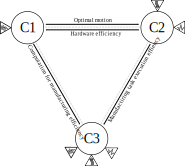
\includegraphics[width=0.9\columnwidth]{fig/grand_challenges_connections_v2.pdf}
	\caption{Interconnection of the different challenges.}
	\label{fig:challengesConnected}
\end{figure}
% ---